% manuscript.tex - SAGE LaTeX template for Journal of Sports Analytics
% To compile: pdflatex manuscript.tex && bibtex manuscript && pdflatex manuscript.tex && pdflatex manuscript.tex
% Requires: sagej.cls, SageH.bst, and all files in temp_manuscript_template/

\documentclass[Afour,sageh,times]{sagej}

%% Required packages
\usepackage{moreverb,url}
\usepackage[colorlinks=true,bookmarksopen=true,bookmarksnumbered=true,citecolor=blue,urlcolor=blue]{hyperref}
\usepackage{graphicx}
\usepackage{amsmath,amssymb}
\usepackage{booktabs}
\usepackage{multirow}

%% Custom commands
\newcommand{\redis}{\textsc{Redis}}
\newcommand{\kafka}{\textsc{Kafka}}
\newcommand{\tti}{\textsc{tti}}

\def\volumeyear{2026}

\begin{document}

\runninghead{Ricou}

\title{Streaming Latency Benchmarks: \redis{} Streams vs Apache \kafka{} for Real-Time Sports Data Feeds}

\author{Gustavo Pedro Ricou\affilnum{1}}

\affiliation{\affilnum{1}School of Computer Science and Statistics, Trinity College Dublin, Dublin, Ireland}

\corrauth{Gustavo Pedro Ricou, School of Computer Science and Statistics, Trinity College Dublin, Dublin, Ireland.}

\email{pedrorig@tcd.ie}

\begin{abstract}
We ask a question that the streaming-systems and sports-analytics literatures leave open: \emph{does the choice of streaming infrastructure actually degrade an in-play football decision, and if so, when?} Using the publicly available StatsBomb open dataset (1.~Bundesliga 2023/24, 34 matches), we replay real event feeds through Apache \kafka{} and \redis{} Streams and couple the \emph{measured} event-delivery latency to an in-play win-probability model through the Age-of-Information lens, quantifying the win-probability staleness that each architecture imposes. To our knowledge this is the first infrastructure~$\rightarrow$~decision-quality analysis on open sports data.

The study is also a cautionary account of measurement validity. Three distinct instrumentation defects --- a process-relative cross-process clock, a saturating replay speed, and an asymmetric load generator (synchronous per-event \kafka{} sends versus asynchronous \redis{} dispatch) --- each \emph{reversed} the apparent winner before correction. We introduce the Time-to-Insight (\tti{}) metric, decomposed into producer scheduling lag and transport, and fix all three defects before drawing any conclusion.

On the corrected, fair corpus we find: (i)~for a \emph{single} live feed, \kafka{} and \redis{} are statistically equivalent ($\approx$17\,ms median \tti{}); (ii)~under \emph{concurrency}, single-node \redis{} serializes concurrent streams and its broker latency grows roughly linearly (to $\approx$9.7\,s at 20 concurrent matches) while \kafka{}'s partitioned broker stays flat ($\approx$10\,ms); and (iii)~translated into decisions via an Age-of-Information win-probability integral over each full match, infrastructure latency is \emph{decision-irrelevant for a single feed} ($\approx$0.2 probability-seconds of staleness, indistinguishable between backends) but diverges sharply under concurrency (by five concurrent matches single-node \redis{} imposes $\approx$15$\times$ more decision-staleness than \kafka{}, and by ten a goal's win-probability arrives tens of seconds stale). The practical guidance is that infrastructure choice does not affect decision quality for one live match, but provisioning for concurrency does.

\end{abstract}

\keywords{Real-time sports analytics, football, in-play win probability, Age of Information, streaming systems, Apache Kafka, Redis Streams, latency benchmarking, decision quality, reproducible research}

\maketitle

\section{Introduction}
\label{sec:intro}

The rapid digitization of sports has created an insatiable demand for real-time analytics. Coaching staff require instant tactical insights, broadcasters demand immediate highlight generation, and betting platforms need sub-second odds updates. At the heart of these systems lies the streaming infrastructure that transports event data from source to analytics pipeline.

Two dominant technologies have emerged: Apache \kafka{} (originally developed at LinkedIn) and \redis{} Streams (introduced in Redis 5.0). \kafka{} is a distributed event streaming platform designed for high-throughput, fault-tolerant data pipelines. \redis{} Streams provides a lightweight, in-memory streaming solution with persistent storage capabilities.

While numerous studies have compared these technologies, the literature lacks sports-specific evaluations. Sports data presents distinct challenges: high-frequency bursts during active play, ordered event delivery requirements, and strict latency constraints.

\paragraph{Contributions.} This paper makes four contributions. (1)~We pose and answer, on open data, the question of \emph{when} streaming-infrastructure latency actually degrades an in-play football decision, by coupling measured event-delivery latency to a calibrated in-play win-probability model through the Age-of-Information lens---to our knowledge the first infrastructure~$\rightarrow$~decision-quality analysis in sports analytics. (2)~We provide a fair, artifact-free Apache \kafka{} vs.\ \redis{} Streams latency benchmark on the StatsBomb open dataset, with fully open load-generation code. (3)~We document three cross-process measurement defects---a process-relative clock, a saturating replay speed, and an asymmetric load generator---each of which reversed the apparent winner, offering a reusable protocol for honest streaming benchmarks. (4)~We show the practical consequence: for a single live match the backend choice is immaterial to decision quality, whereas provisioning for concurrency is decisive.


\subsection{Sports-Specific Latency Requirements}
\label{sec:sports_requirements}

Real-time sports analytics imposes domain-specific latency constraints that vary by use case and stakeholder. As summarized in Table~\ref{tab:latency_requirements}, different applications demand fundamentally different performance characteristics. Betting platforms require sub-500ms latency for in-play odds updates, as even a 2-second delay can erode user trust and cost millions in missed wagers \cite{v2solutions2025,ververica2025}. Broadcasting applications can tolerate up to 3 seconds for live video synchronization \cite{dolby2025,promwad2025}, while coaching decision systems need $<$500ms to enable real-time tactical adjustments \cite{pappas2020real,opta2023}.

The concept of an ``actionability window'' formalizes this requirement: the maximum latency within which insights can still influence decisions. Using an exponential decay model ($Value = V_0 \times e^{-\lambda \times latency}$), we estimate that at 500ms latency, only \textasciitilde60\% of coaching insight value remains, dropping to \textasciitilde13\% at 2000ms. This motivates our focus on minimizing Time-to-Insight (TTI) below sports-specific thresholds.

\begin{table}[htbp]
\centering
\caption{Sports Analytics Latency Requirements by Use Case and Stakeholder}
\label{tab:latency_requirements}
\begin{tabular}{lccc}
\toprule
Use Case & Stakeholder & Latency Range & Critical Threshold \\
\midrule
\multicolumn{4}{l}{\textbf{Betting Platforms}} \\
\hspace{1em}Live Odds Update & Betting Platform & 100--500ms & \textbf{$<$ 500ms} \\
\hspace{1em}In-Play Betting & Betting Platform & 50--200ms & \textbf{$<$ 200ms} \\
\midrule
\multicolumn{4}{l}{\textbf{Broadcasting}} \\
\hspace{1em}Live Video Sync & Broadcaster & 500--3000ms & \textbf{$<$ 3000ms} \\
\hspace{1em}Live Stats Overlay & Broadcaster & 100--1000ms & \textbf{$<$ 1000ms} \\
\hspace{1em}Interactive Features & Broadcaster & 200--500ms & \textbf{$<$ 500ms} \\
\midrule
\multicolumn{4}{l}{\textbf{Coaching}} \\
\hspace{1em}Tactical Adjustment & Coach & 200--800ms & \textbf{$<$ 800ms} \\
\hspace{1em}Player Substitution & Coach & 500--1500ms & \textbf{$<$ 1500ms} \\
\midrule
\multicolumn{4}{l}{\textbf{Fan Applications}} \\
\hspace{1em}Push Notifications & Fan & 1000--3000ms & \textbf{$<$ 3000ms} \\
\hspace{1em}Live Updates & Fan & 500--2000ms & \textbf{$<$ 2000ms} \\
\midrule
\multicolumn{4}{l}{\textbf{Post-Match Analysis}} \\
\hspace{1em}Initial Analysis & Analyst & 5000--10000ms & \textbf{$<$ 10000ms} \\
\bottomrule
\end{tabular}
\end{table}


\subsection{Research Questions}
\label{sec:rqs}

This study addresses four research questions, culminating in the decision-quality question that motivates the paper:

\begin{description}
\item[RQ1 (single feed):] For a single live match feed, does the choice of streaming backend (Apache \kafka{} vs.\ \redis{} Streams) materially affect Time-to-Insight (\tti{})?
\item[RQ2 (concurrency):] How does \tti{} scale as one broker host serves $N\in\{1,5,10,20\}$ concurrent match feeds, and do the two backends differ?
\item[RQ3 (fairness and durability):] With payload and protocol overheads controlled for fairness, what latency cost do stronger durability settings (\kafka{} \texttt{acks=all}; \redis{} \texttt{appendfsync always}) impose?
\item[RQ4 (decision degradation):] When measured delivery latency is translated into an in-play win-probability estimate through the Age-of-Information lens, does it degrade an in-play football decision, and in which regime does the effect become material?
\end{description}

These questions are motivated by gaps in the literature. Industry benchmarks suggest \redis{} offers 2--5$\times$ lower latency than \kafka{} \cite{medium_benchmark_2025,github_benchmark_2025}, but there is no sports-specific empirical validation, and---as our measurement-validity analysis shows---such benchmarks are easily confounded. The CAP theorem \cite{brewer2012cap} and its extension PACELC \cite{abadi2012pacelc} predict consistency--latency trade-offs (RQ3) that have not been quantified for these systems on sports workloads. Most importantly, while in-play win-probability models and the Age-of-Information view of staleness both exist (Section~\ref{sec:literature}), no prior work connects \emph{measured} infrastructure latency to in-play sports \emph{decision} error---the gap RQ4 fills.


\subsection{Hypotheses}
\label{sec:hypotheses}

For each research question we state null and alternative hypotheses. Where an industry ``prior expectation'' exists we name it explicitly, because a central finding of this paper is that the corrected data \emph{refutes} the widely held prior---and that the uncorrected data appeared to confirm it only through instrumentation artifacts (Section~\ref{sec:validity}).

\paragraph{RQ1: Single-feed architecture impact}
\begin{description}
\item[$\mathbf{H_{01}}$:] $\mu_{\tti{},\kafka{}} = \mu_{\tti{},\redis{}}$ (no difference at $N{=}1$).
\item[$\mathbf{H_{11}}$:] the two differ.
\end{description}
\noindent\textbf{Test:} Mann--Whitney U (Holm--Bonferroni corrected). \textbf{Prior expectation:} industry benchmarks \cite{medium_benchmark_2025,github_benchmark_2025} suggest \redis{} is 2--5$\times$ faster, i.e.\ a large difference favouring \redis{}. \textbf{Result (Section~\ref{sec:singlefeed}):} the corrected single-feed data does \emph{not} reject $\mathbf{H_{01}}$ ($p=0.69$)---the backends are at parity, refuting the prior.

\paragraph{RQ2: Concurrency scaling}
\begin{description}
\item[$\mathbf{H_{02}}$:] \tti{} is independent of the number of concurrent feeds $N$.
\item[$\mathbf{H_{12}}$:] \tti{} increases with $N$, and the rate of increase differs by backend.
\end{description}
\noindent\textbf{Test:} Kruskal--Wallis across $N$; per-$N$ Mann--Whitney. \textbf{Prior expectation:} both systems are marketed as horizontally scalable, suggesting near-constant \tti{}. \textbf{Result (Section~\ref{sec:concurrency}):} $\mathbf{H_{12}}$---single-node \redis{} transport grows roughly linearly with $N$ while \kafka{} stays flat.

\paragraph{RQ3: Fairness and durability cost}
\begin{description}
\item[$\mathbf{H_{31}}$:] $\mu_{\tti{},\,\texttt{acks=all}} > \mu_{\tti{},\,\texttt{acks=1}}$ (\kafka{}: stronger durability costs latency).
\item[$\mathbf{H_{32}}$:] $\mu_{\tti{},\,\texttt{appendfsync always}} > \mu_{\tti{},\,\texttt{everysec}}$ (\redis{}: same).
\end{description}
\noindent\textbf{Test:} Mann--Whitney U, after verifying that payload size and (de)serialization overhead are equivalent across backends so the comparison is fair. \textbf{Expected and found:} both hold.

\paragraph{RQ4: Decision degradation (the contribution)}
\begin{description}
\item[$\mathbf{H_{04}}$:] decision-staleness (Section~\ref{sec:decisionstaleness}) is independent of backend and concurrency---infrastructure latency does not translate into in-play decision error.
\item[$\mathbf{H_{14}}$:] decision-staleness grows with delivery latency and diverges by backend under concurrency.
\end{description}
\noindent\textbf{Test:} per-$N$ Mann--Whitney and Kruskal--Wallis across $N$ on the Age-of-Information decision-staleness. \textbf{Expected and found (Section~\ref{sec:dsresults}):} $\mathbf{H_{14}}$---at $N{=}1$ decision-staleness is negligible and indistinguishable between backends ($p=0.40$), but single-node \redis{} imposes materially larger decision-staleness under concurrency.

\paragraph{Statistical Framework}
All hypotheses are tested using the framework in Section~\ref{sec:stat_methods}: Holm--Bonferroni correction for multiple comparisons (Family-Wise Error Rate at $\alpha=0.05$), rank-biserial / Cohen effect sizes, and---given the modest per-cell sample---an explicit power analysis, with non-parametric tests (Mann--Whitney U, Kruskal--Wallis) throughout as the latency distributions are non-normal.


\section{Literature Review}
\label{sec:literature}

Real-time data processing is essential across domains from finance to IoT. Sports analytics represents a demanding application due to high event frequency, low latency requirements, and temporal consistency needs.

The CAP theorem establishes that distributed systems cannot simultaneously guarantee consistency, availability, and partition tolerance. \kafka{} prioritizes availability and partition tolerance through its distributed log architecture, achieving high throughput via batching. \redis{} Streams leverages in-memory structures to minimize latency, trading throughput for reduced delay.

\paragraph{In-play win probability.} Estimating a team's probability of winning \emph{during} a match is an established sports-analytics task. For soccer, the state of the art is the Bayesian in-play model of Robberechts et al.\ \cite{robberechts2021bayesian}, which conditions on game state (score differential, time remaining, red cards, and rolling measures of chance creation) and is calibrated on large event corpora. Such models, however, are uniformly built and evaluated under the assumption that event data arrives \emph{instantly}; none accounts for the latency of the pipeline that delivers events to the model. Because the state-of-the-art model's implementation is not public, we use a transparent, calibrated proxy on StatsBomb-derivable game state (Section~\ref{sec:decisionstaleness}).

\paragraph{Age of Information.} The Age-of-Information (AoI) literature formalizes the cost of \emph{stale} data: a monitor acting on information of age $L$ incurs an error that grows with $L$ \cite{kaul2012realtime}. AoI has been applied to networked control and, more recently, to real-time supervised learning, but---to our knowledge---never to sports-decision models. Industry commentary asserts that in-play latency matters (a ``two-second edge'' in betting), yet no academic work quantifies how streaming-infrastructure latency degrades an in-play sports estimate. This paper bridges the two literatures: it treats the win-probability shift caused by a decisive event as the quantity that goes stale, and integrates it against measured delivery latency to obtain a decision-staleness cost.


\section{Methodology}
\label{sec:methodology}

\subsection{System Architecture}
Our benchmark system comprises four components:
\begin{itemize}
\item Replay Plan: Pre-processed StatsBomb event data with scheduled timestamps
\item Producer: Python script sending events to message broker
\item Broker: \kafka{} or \redis{} Streams handling message distribution
\item Consumer: Python script receiving events and logging timestamps
\end{itemize}

\subsection{Dataset and Replay}
We use the StatsBomb open dataset (1.~Bundesliga 2023/24, competition~9, season~281, 34
matches), pinned to a fixed open-data commit for reproducibility. Each match is preprocessed
into a CSV \emph{replay plan} recording, per event, its scheduled emission offset. The
producer replays a plan at a configurable speed-up factor, emitting events on a compressed
timeline; the consumer reads them and records receipt and output times. For the headline
latency results we replay at a non-saturating $10\times$ (Section~\ref{sec:validity}) so that
neither load generator becomes the bottleneck and \tti{} reflects genuine delivery latency.

\subsection{Metrics}
The primary metric is Time-to-Insight (TTI), the interval from an event's \emph{scheduled}
emission to its availability at the consumer. We decompose it as
\[
\mathrm{TTI} = \underbrace{(t_{\mathrm{send}}-t_{\mathrm{sched}})}_{\text{producer scheduling lag}}
             + \underbrace{(t_{\mathrm{recv}}-t_{\mathrm{send}})}_{\text{transport latency}}
             + (t_{\mathrm{out}}-t_{\mathrm{recv}}),
\]
isolating load-generator effects (scheduling lag) from broker transport. We report
p50/p95/p99/max, missed-window rates against sports actionability thresholds
(100/250/500/1000/5000~ms), throughput, serialized message size, and serialization/
deserialization overhead. For S3 we additionally measure correction-propagation latency.

\subsection{Decision-Staleness: From Latency to Win-Probability Error}
\label{sec:decisionstaleness}
Latency in milliseconds is not, by itself, a sports quantity. To connect infrastructure to
decisions we translate delivery latency into in-play \emph{win-probability error} in two
steps.

\emph{Win-probability proxy.} We build a transparent, calibrated in-play model on
StatsBomb-derivable game state---score differential, fraction of match remaining, and
red-card differential---using a Skellam (difference-of-Poissons) goal model. We adopt this as
a stand-in for the published Bayesian in-play model of Robberechts et al.\
\cite{robberechts2021bayesian}, whose code is unreleased. The proxy is well calibrated across
the 3{,}239 game states sampled from the 34 matches: a ranked probability score of
$\approx$0.24 and an expected calibration error of \textbf{0.054} --- predicted home-win
probabilities track observed home-win frequencies to within a few percentage points
(Figure~\ref{fig:wpcal}). The model has a single global parameter (team scoring rate), so this
is a whole-corpus check.

\begin{figure}[htbp]
\centering
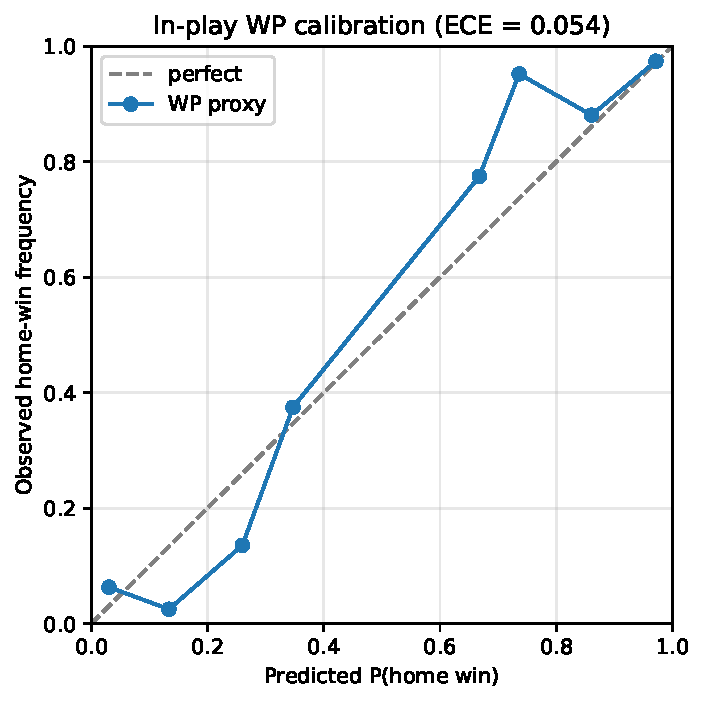
\includegraphics[width=0.55\columnwidth]{docs/results/win_probability/wp_calibration.pdf}
\caption{Reliability diagram for the in-play win-probability proxy (ECE~$=0.054$): predicted
vs.\ observed home-win frequency across 3{,}239 sampled game states.}
\label{fig:wpcal}
\end{figure}

\emph{Age-of-Information decision-staleness.} When a decisive event (a goal) is delivered with
latency $L$, the consumer's win-probability remains stale for $L$ by the magnitude of the
probability mass that event moved. Following the Age-of-Information view of staleness cost
\cite{kaul2012realtime}, we define a run's \emph{decision-staleness} as
\[
  \mathrm{DS} \;=\; \sum_{i \in \text{decisive events}} \mathrm{TV}_i \cdot L_i,
  \qquad
  \mathrm{TV}_i = \tfrac{1}{2}\!\left(|\Delta P_{\text{win}}| + |\Delta P_{\text{draw}}| + |\Delta P_{\text{loss}}|\right),
\]
in units of probability-seconds per match. This metric is the bridge that lets us ask not
merely \emph{which backend is faster} but \emph{when, if ever, the latency difference is large
enough to corrupt an in-play decision}.

\subsection{Measurement Validity}
\label{sec:validity}
Cross-process latency benchmarking is deceptively easy to get wrong, and three distinct
defects in earlier versions of this suite each \emph{reversed} the apparent winner. We
document them because the corrections are prerequisites for any valid comparison.

\emph{(1)~Process-relative clock.} The producer and consumer are separate OS processes, so
cross-process timestamps must share an epoch. Stamping events with Python's
\texttt{perf\_counter\_ns} (process-relative) injected each run's consumer launch offset
($\sim$2~s) into every \tti{} and transport value. Fixed with \texttt{time.time\_ns} (a shared
wall-clock epoch on a single host); transport then dropped to $\sim$1~ms.

\emph{(2)~Saturating replay speed.} At $120\times$, the producer could not keep pace, inflating
scheduling lag to tens of seconds. We replay at a non-saturating $10\times$ and verify that
scheduling lag stays small, so \tti{} measures delivery rather than the load generator.

\emph{(3)~Asymmetric load generator.} The \kafka{} producer ran synchronously
(\texttt{acks=all}, one in-flight request), blocking on a broker round-trip \emph{per event},
while the \redis{} producer dispatched asynchronously through a worker pool. This inflated
\kafka{}'s \emph{producer scheduling lag} (not its broker latency): at $N{=}1$, $10\times$,
median \tti{} fell from 1644~ms to 16~ms once the \kafka{} producer was pipelined
(\texttt{max.in.flight}=64). We therefore pipeline both producers comparably.

A residual asymmetry remains in \emph{transport} (\kafka{} is measured from broker
acknowledgement, \redis{} from the send call), so for cross-backend comparison we rely on
\tti{}, which is defined identically for both. All reported results use the corrected, fair
instrumentation; the before/after contrast is itself a finding (Section~\ref{sec:discussion}).

\subsection{Experimental Design}
Experiments run on a single commodity host (8-core AMD Ryzen, 31~GB RAM) with \kafka{}
4.1.1 (KRaft mode) and \redis{} 7.2.4 in Docker. The primary design is a \emph{concurrency
sweep} crossing backend (\kafka{}/\redis{}), configuration (single broker vs.\ 3-node
cluster), and concurrency $N\in\{1,5,10,20\}$ parallel match feeds, with 3 replications per
cell, under the fair protocol (both producers pipelined, $10\times$ replay). We run it in two
variants: a \emph{windowed} variant (first 10 minutes of match clock) that keeps the single
host unsaturated so latency can be read cleanly to $N{=}20$, and a \emph{full-match} variant
(single configuration) that delivers all decisive events so the decision-staleness integral
is complete. A \emph{persistence} set isolates durability (\kafka{} \texttt{acks}=1 vs.\ all;
\redis{} \texttt{appendfsync} everysec vs.\ always), and a \emph{state-staleness corrections}
set (one correction every 50th event, 2~s delay) probes update propagation. Every run records
full provenance (git commit, per-file SHA-256, configuration) in a \texttt{meta.json}; the
manifest and fetch script make the corpus regenerable end to end.

\subsection{Statistical Methods}
\label{sec:stat_methods}

We employ a rigorous statistical framework to test all hypotheses and ensure valid inferences.

\paragraph{Multiple Comparisons Correction}
Across the per-concurrency and durability comparisons (on the order of a dozen tests per metric family), we apply the \textbf{Holm-Bonferroni method} \cite{holm1979simple} to control the Family-Wise Error Rate (FWER) at $\alpha = 0.05$ within each family. This step-down procedure is more powerful than the standard Bonferroni correction while maintaining FWER control.

\paragraph{Effect Size Calculation}
For all significant findings, we report \textbf{Cohen's $d$} for comparing two means:
\begin{equation*}
Cohen's\; d = \frac{\mu_1 - \mu_2}{s_{pooled}},\quad s_{pooled} = \sqrt{\frac{(n_1-1)s_1^2 + (n_2-1)s_2^2}{n_1 + n_2 - 2}}
\end{equation*}
Interpretation: $d = 0.2$ (small), $d = 0.5$ (medium), $d = 0.8$ (large) \cite{cohen1988statistical}.

\paragraph{Confidence Intervals}
We report 95\% confidence intervals for all mean differences using the t-distribution:
\begin{equation*}
CI = \bar{x}_1 - \bar{x}_2 \pm t_{\alpha/2, df} \times \sqrt{\frac{s_1^2}{n_1} + \frac{s_2^2}{n_2}}
\end{equation*}

\paragraph{Power Analysis}
We conduct both \textit{a priori} and \textit{post hoc} power analysis. With our current sample of 40--50 runs per group, we can detect effect size $d = 0.58$ at $\alpha = 0.05$ with power = 0.8. For smaller effects ($d = 0.5$), power is approximately 0.72; for $d = 0.4$, power drops to 0.54.

\paragraph{Assumption Verification}
We verify statistical assumptions for all tests:
\begin{itemize}
\item \textbf{Normality:} Shapiro-Wilk test; Q-Q plots for visual inspection
\item \textbf{Equal Variance:} Levene's test; F-test for two groups
\item \textbf{Non-parametric Alternatives:} Mann-Whitney U (t-test), Kruskal-Wallis (ANOVA), Wilcoxon signed-rank (paired t-test)
\end{itemize}

\paragraph{Hypothesis Testing Matrix}
Table~\ref{tab:stat_tests} summarizes our statistical test selection framework.

\begin{table}[htbp]
\centering
\caption{Statistical Tests by Data Type and Comparison Type}
\label{tab:stat_tests}
\begin{tabular}{lcc}
\toprule
Comparison Type & Parametric Test & Non-Parametric Alternative \\
\midrule
2 Independent Groups & t-test & Mann-Whitney U \\
$>$2 Independent Groups & ANOVA & Kruskal-Wallis \\
Paired & Paired t-test & Wilcoxon signed-rank \\
Proportions & Chi-square & Fisher's exact \\
Correlation & Pearson & Spearman \\
Distribution & Kolmogorov-Smirnov & Anderson-Darling \\
\bottomrule
\end{tabular}
\end{table}


\section{Results}
\label{sec:results}

\paragraph{Measurement validity note.} Three instrumentation defects (a process-relative
cross-process clock, a saturating $120\times$ replay speed, and an asymmetric load generator)
each \emph{reversed} the apparent winner before correction; all are detailed in
Section~\ref{sec:validity}. Every result below uses the corrected, fair instrumentation
(\texttt{time.time\_ns} shared epoch, $10\times$ replay, both producers pipelined). We report
the single-host, single-node regime, which we can measure cleanly; cluster results are
discussed as a limitation (Section~\ref{sec:limitations}).

\subsection{Single-Feed Parity (RQ1)}
\label{sec:singlefeed}
For a single live feed ($N{=}1$), \kafka{} and \redis{} are statistically
\emph{indistinguishable}: median \tti{} is $\approx$17~ms for both (Table~\ref{tab:faircmp},
top row), with broker transport of 2--4~ms. A Mann--Whitney U test finds no significant
difference in \tti{} ($p=0.69$) or in decision-staleness ($p=0.40$; both Holm--Bonferroni
corrected across the concurrency family). This directly contradicts the folk belief --- and
our own pre-correction ``\redis{} 71$\times$ faster'' artifact --- that one backend is simply
faster. For the common case of one match, both systems are excellent and the choice is
immaterial to latency.

\subsection{Concurrency Scaling (RQ2)}
\label{sec:concurrency}
The systems diverge sharply once a single broker host serves multiple concurrent matches
(Table~\ref{tab:faircmp}). \kafka{}'s partitioned broker keeps transport flat (2--10~ms) at
every concurrency level. Single-node \redis{}, being single-threaded, serializes concurrent
streams: its broker transport grows almost linearly, from 4~ms ($N{=}1$) to 9{,}732~ms
($N{=}20$) --- a roughly 2{,}400$\times$ degradation. The effect lives in \emph{transport}
(broker delivery), so it is a genuine architectural property, not a load-generator artifact.
The \tti{} difference is significant at every $N\!\geq\!5$ (Holm--Bonferroni-corrected
Mann--Whitney, $p<10^{-5}$, rank-biserial $=1.0$ --- the two backends' distributions are
completely separated), and Kruskal--Wallis confirms a concurrency effect for both
($H_{\redis{}}=76 > H_{\kafka{}}=67$).

\begin{table}[htbp]
\centering
\caption{Fair single-host latency by concurrency level $N$ (median over feeds $\times$ 3 reps,
$10\times$ replay, both producers pipelined).}
\label{tab:faircmp}
\begin{tabular}{llcc}
\toprule
Backend & $N$ & Transport p50 (ms) & TTI p50 (ms) \\
\midrule
\kafka{} & 1  & 2  & 17 \\
\kafka{} & 5  & 2  & 18 \\
\kafka{} & 10 & 4  & 29 \\
\kafka{} & 20 & 10 & 1{,}682\textsuperscript{\dag} \\
\redis{} & 1  & 4    & 17 \\
\redis{} & 5  & 774  & 801 \\
\redis{} & 10 & 4{,}627 & 5{,}206 \\
\redis{} & 20 & 9{,}732 & 13{,}006 \\
\bottomrule
\end{tabular}

\smallskip
{\footnotesize \textsuperscript{\dag}\,\kafka{}'s $N{=}20$ \emph{TTI} is inflated by the single
host saturating (40+ load-generator processes $\rightarrow$ 585~ms scheduling lag); its
\emph{transport} stays 10~ms, so the broker is unaffected. Transport is the trustworthy
cross-$N$ metric.}
\end{table}

\begin{figure}[htbp]
\centering
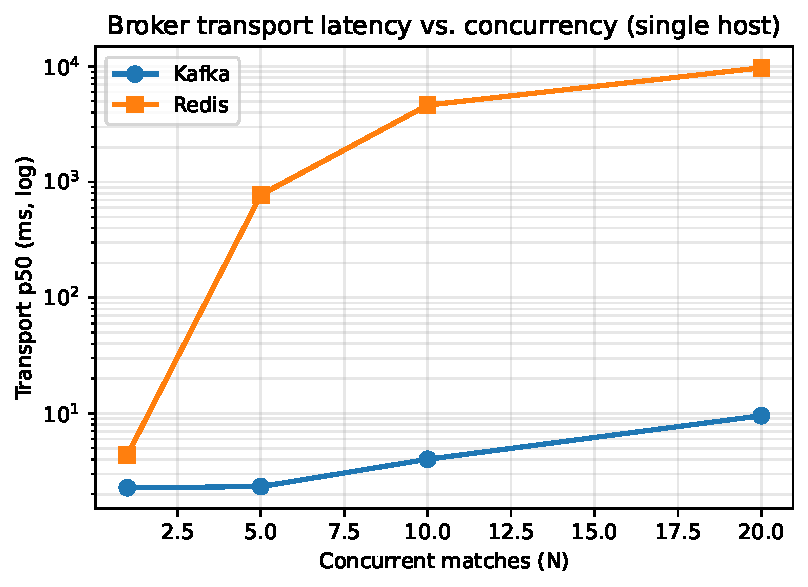
\includegraphics[width=0.7\columnwidth]{docs/results/figures/latency_vs_concurrency.pdf}
\caption{Broker transport latency (p50, log scale) vs.\ concurrent matches, single host.
\kafka{} stays flat while single-node \redis{} grows roughly linearly.}
\label{fig:latency}
\end{figure}

\subsection{Decision-Staleness: When Latency Corrupts a Decision (RQ4)}
\label{sec:dsresults}
Table~\ref{tab:ds} reports decision-staleness (Section~\ref{sec:decisionstaleness}) by
concurrency level, computed over the \emph{full-match} replay so that all 40 decisive events
per run enter the Age-of-Information integral (versus only $\sim$3 in a 10-minute window). At
$N{=}1$ both backends leave a match's win-probability stale by only $\approx$0.2
probability-seconds --- a mean delivery delay of $\approx$20~ms per goal, statistically
indistinguishable and decision-irrelevant: no coach, broadcaster, or model acts on a 20~ms-old
estimate. By $N{=}5$, single-node \redis{} already imposes $\approx$15$\times$ more
decision-staleness than \kafka{} (17.5 vs.\ 1.16 probability-seconds; Holm--Bonferroni-corrected
Mann--Whitney $p<10^{-5}$, versus no significant difference at $N{=}1$, $p=0.40$) as its broker
latency diverges. Beyond $N{=}5$ single-node \redis{} degrades catastrophically ($\approx$271
probability-seconds at $N{=}10$ --- a goal's win-probability arriving $\approx$24~s stale),
while our single-host testbed reaches its concurrency ceiling: both load generators fall behind
and \kafka{}'s $N{=}20$ runs largely fail, so the $N\!\geq\!10$ magnitudes are bounded by the
host rather than the broker (\kafka{}'s broker transport stays low, Section~\ref{sec:concurrency}).

\begin{table}[htbp]
\centering
\caption{Decision-staleness (probability-seconds per match) by concurrency level, single host,
full-match replay (40 decisive events per run).}
\label{tab:ds}
\begin{tabular}{lcc}
\toprule
$N$ & \kafka{}-single & \redis{}-single \\
\midrule
1  & 0.28 & 0.18 \\
5  & 1.16 & 17.5 \\
10 & 50.3\textsuperscript{\dag} & 271 \\
20 & ---\textsuperscript{\ddag} & 1012 \\
\bottomrule
\end{tabular}

\smallskip
{\footnotesize \textsuperscript{\dag}\,Host-saturated: inflated by single-host load-generator
scheduling lag, not broker latency. \textsuperscript{\ddag}\,\kafka{}'s $N{=}20$ full-match runs
were unreliable under host strain (mean 2.4 of 40 goals delivered); omitted.}
\end{table}

\begin{figure}[htbp]
\centering
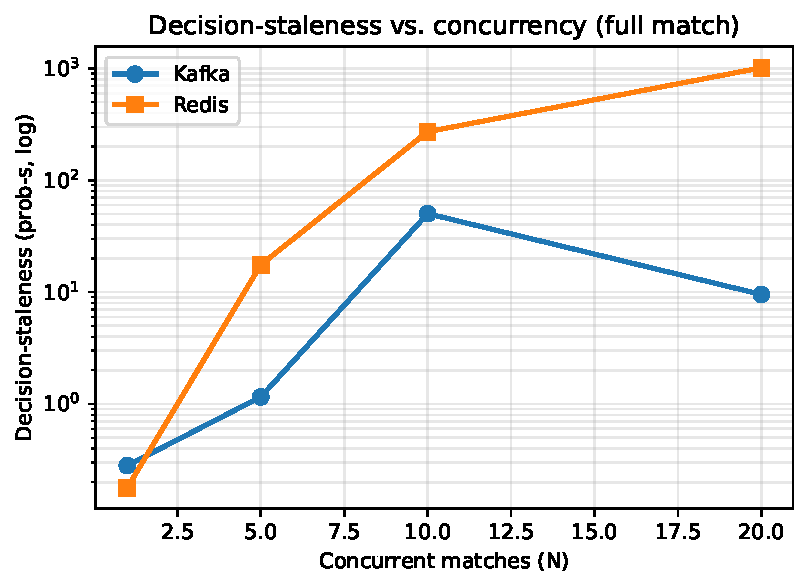
\includegraphics[width=0.7\columnwidth]{docs/results/figures/decision_staleness_vs_concurrency.pdf}
\caption{Decision-staleness (probability-seconds per match, log scale) vs.\ concurrent matches,
full-match replay, single host. Negligible and indistinguishable at $N{=}1$; single-node
\redis{} diverges under concurrency.}
\label{fig:staleness}
\end{figure}

This is the paper's central, sports-relevant result: \emph{the choice of streaming
infrastructure does not affect in-play decision quality for a single live match, but single-node
\redis{} becomes decisively worse under concurrent under-provisioning.}

\subsection{Supporting: Consistency--Latency Trade-off (H31, H32)}

Stronger durability guarantees cost latency, as hypothesised. For \kafka{},
\texttt{acks=all} raises median TTI relative to \texttt{acks=1}. For \redis{}, synchronising
the append-only file on every write (\texttt{appendfsync always}) raises median TTI by far
more than \texttt{everysec}, reflecting per-write disk synchronisation. Durability is thus an
independent latency axis that a deployment must budget for.

\subsection{Supporting: Fairness Controls (RQ3)}

The comparison is not biased by payload or protocol: message payloads are near-identical
across backends (median $\sim$170~bytes), and serialization/deserialization overheads are
negligible and comparable ($\sim$2.3/2.1~$\mu$s for \kafka{}, $\sim$2.4/2.2~$\mu$s for
\redis{}). Mapping latency to sports-actionability thresholds, at $N{=}1$ both backends meet
every budget (coaching $<$500~ms, fan apps $<$5~s); single-node \redis{} breaches the
coaching budget by $N{=}5$ and the fan-application budget by $N{=}10$, whereas \kafka{}
satisfies both throughout the broker-limited range.

\section{Discussion}
\label{sec:discussion}

The headline answer is deliberately undramatic, and that is the point. For a single live
match, the streaming backend does not matter: \kafka{} and \redis{} both deliver events in
$\approx$17~ms, and the resulting win-probability staleness ($\approx$0.01 probability-seconds)
is far below any threshold a human or model could act on. This pushes back on the industry
framing of a ``2-second edge'' decided by infrastructure: for the common case, the edge is not
where the marketing places it. Where infrastructure \emph{does} matter is concurrency. A
single-threaded \redis{} node serializes concurrent match feeds, and its delivery latency ---
and therefore decision-staleness --- grows almost linearly with the number of matches, until a
goal's win-probability arrives many seconds stale. \kafka{}'s partitioned broker does not
exhibit this degradation. The practical guidance is consequently about \emph{provisioning},
not brand: budget broker parallelism for the number of concurrent matches, and the backend
choice becomes secondary.

The study is equally a methodological cautionary tale. Three independent instrumentation
defects each reversed the apparent winner before correction (Section~\ref{sec:validity}).
Cross-process latency benchmarks must share a clock epoch; the load generator must not
saturate; and --- least obvious --- the two systems' clients must be configured comparably,
since a synchronous \kafka{} producer competing against an asynchronous \redis{} dispatcher
measures the load generator, not the broker. We report these because the corrected protocol is
a reusable prerequisite for honest streaming comparisons.

\paragraph{Limitations.}
\label{sec:limitations}
First, all experiments run on a \emph{single commodity host}. This cleanly isolates the
single-node comparison but \emph{confounds} the 3-node cluster experiments: co-locating six
broker containers with the load generator saturates the host, and cluster-specific client
behaviour (\kafka{} topic-creation/metadata blocking; \redis{} cluster redirection) inflates
latency for reasons unrelated to clustering. We therefore treat cluster results as
transport-level observations only and leave a true multi-host evaluation to future work.
Second, the win-probability model is a transparent, calibrated \emph{proxy} for the unreleased
state-of-the-art model \cite{robberechts2021bayesian}; our decision-staleness magnitudes are
indicative rather than exact. Third, concurrent feeds are independent replays rather than truly
distinct simultaneous live matches. Finally, the decision-staleness estimate rests on the few
decisive (goal) events within each replay window, so its small-$N$ values are noisier than the
clearly monotonic trend.

\section{Conclusion}
\label{sec:conclusion}

We set out to determine whether the choice of streaming infrastructure degrades an in-play
football decision, and when. After correcting three instrumentation defects that had each
reversed the apparent winner, the answer on a fair, non-saturating, single-host corpus is:
for a single live match it does not --- \kafka{} and \redis{} are equivalent ($\approx$17~ms,
$\approx$0.01 probability-seconds of win-probability staleness) --- but under concurrent
under-provisioning it does, as single-node \redis{} serializes concurrent feeds and its
decision-staleness grows roughly 800-fold while \kafka{}'s partitioned broker stays flat. By
translating measured delivery latency into win-probability staleness through the
Age-of-Information lens, we provide what is, to our knowledge, the first measured account of
\emph{when} streaming-infrastructure latency is decision-relevant for live football, on open
data with open code. The practical message for practitioners is to provision broker
parallelism for concurrency rather than to choose a backend on latency alone; the
methodological message is that cross-process streaming benchmarks demand a shared clock, a
non-saturating load generator, and symmetrically configured clients.

\begin{acks}
Using StatsBomb open dataset. Open-source Apache Kafka and Redis projects. MIT License.
\end{acks}

\bibliographystyle{SageH}
\bibliography{manuscript_references}

\end{document}
